\documentclass{standalone}
\usepackage{tikz}
\usetikzlibrary{calc,positioning,backgrounds}
\begin{document}
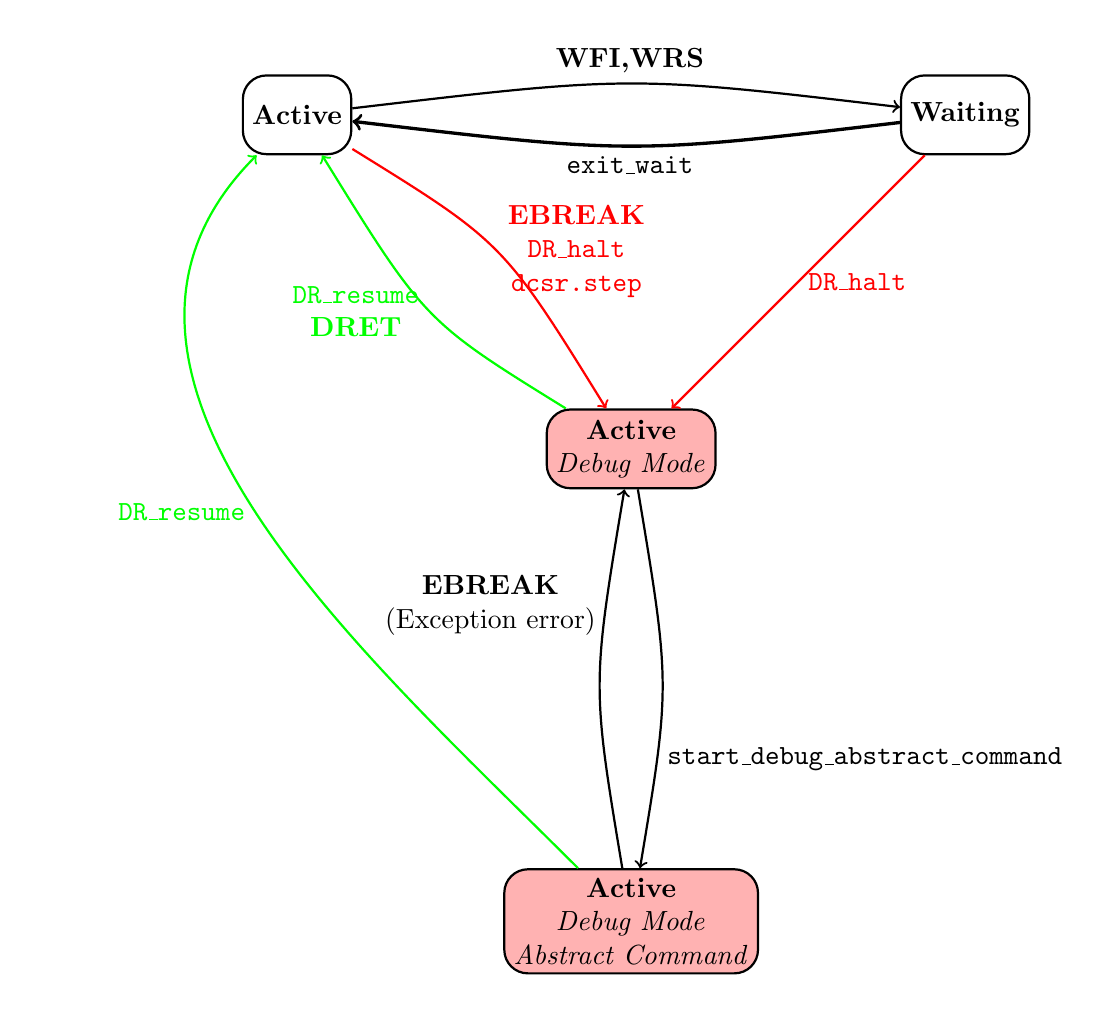
\begin{tikzpicture}[
    % these two lines are needed for the svg to receive a white background.
    background rectangle/.style={rounded corners,fill=white},
    framed,
    % general settings
    node distance=6cm,
    align=center,
    % nodes
    base/.style={rectangle, rounded corners=3mm, minimum size=10mm, thick, draw=black},
    wait/.style={base, draw=black},
    debug/.style={base, draw=black, fill=red!30},
    % arrow labels
    label/.style={text=black},
    hltlabel/.style={text=red},
    reslabel/.style={text=green},
    % arrows
    enterwait/.style={black, thick},
    exitwait/.style={black, very thick},
    halt/.style={red, thick},
    resume/.style={green, thick},
    dbgarr/.style={black, thick},
  ]

  \node (dbg)      [debug]                             {\textbf{Active}\\
                                                        \textit{Debug Mode}};

  \node (active)   [base, above left  of=dbg]          {\textbf{Active}};
  \node (wait)     [wait, above right of=dbg]          {\textbf{Waiting}};

  \node (dbg-cmd)  [debug, below of=dbg]               {\textbf{Active}\\
                                                        \textit{Debug Mode}\\
                                                        \textit{Abstract Command}};

  % not used anymore.
  %\node (dbg-err)  [debug, below right of=dbg]         {\textbf{Active}\\
  %                                                      \textit{Debug Mode}\\
  %                                                      \textit{Abstract Command Error}};

  % control for enterwait arrow
  \coordinate (nwaitloc) at ($(active)!0.5!(wait)+(0,0.5cm)$);
  % control for exitwait arrow
  \coordinate (xwaitloc) at ($(active)!0.5!(wait)-(0,0.5cm)$);

  \draw[->,enterwait] (active) .. controls (nwaitloc) .. node[label,above]{\textbf{WFI,WRS}}      (wait);
  \draw[->,exitwait]  (wait)   .. controls (xwaitloc) .. node[label,below]{\texttt{exit\_wait}}   (active);

  % control for halt-active arrow
  \coordinate (haltactloc) at ($(active)!0.5!(dbg)+(0.5cm,0.5cm)$);
  % control for resume arrow
  \coordinate (resumeloc) at ($(active)!0.5!(dbg)-(0.5cm,0.5cm)$);

  \draw[->,halt]   (active)  .. controls (haltactloc) .. node[hltlabel,right]{\textbf{EBREAK}\\\texttt{DR\_halt}\\\texttt{dcsr.step}} (dbg);
  \draw[->,halt]   (wait)    -- node[hltlabel,right]{\texttt{DR\_halt}}                                           (dbg);
  \draw[->,resume] (dbg)     .. controls (resumeloc)  .. node[reslabel,left]{\texttt{DR\_resume}\\\textbf{DRET}}     (active);

  % control for start-cmd arrow
  \coordinate (startcmdloc) at ($(dbg)!0.5!(dbg-cmd)+(0.5cm,0)$);
  % control for end-cmd arrow
  \coordinate (endcmdloc)   at ($(dbg)!0.5!(dbg-cmd)-(0.5cm,0)$);

  \draw[->,dbgarr] (dbg)     .. controls (startcmdloc) .. node[label,right, near end]{\texttt{start\_debug\_abstract\_command}} (dbg-cmd);
  \draw[->,dbgarr] (dbg-cmd) .. controls (endcmdloc)   .. node[label,left, near end]{\textbf{EBREAK}\\(Exception error)}        (dbg);

  \draw[->,resume] (dbg-cmd) edge [out=135,in=-135] node[reslabel,left]{\texttt{DR\_resume}}                                    (active);

\end{tikzpicture}
\end{document}
